\documentclass[a4paper]{article}
\usepackage[top=1in,bottom=1in,left=1in,right=1in]{geometry}
\usepackage{times}
\usepackage{amssymb}
\usepackage{mathtools}	% pulls in amsmath
	\mathtoolsset{centercolon}
\usepackage{tikz}
	\usetikzlibrary{automata}
	\usepackage{tikz-qtree}
\usepackage{mathpartir}
\usepackage{amsthm}
\usepackage{amsxtra}
\usepackage{algorithm}
\usepackage{algpseudocode}
\usepackage{semantic}
	\reservestyle{\declarevars}{\texttt}
	\reservestyle{\declareops}{\texttt}
	\reservestyle{\declarestates}{\text}
\usepackage{color}
\usepackage{listings}
\usepackage{mathtools}
\usepackage[shortlabels]{enumitem}
\usepackage{graphicx}	% for pdf image

\newtheorem{theorem}{Theorem}

\newtheorem{myexample}{\textbf{Example}}
\newtheorem{mylemma}{\textbf{Lemma}}
\newtheorem{myproof}{\textbf{Proof}}
\newtheorem{myinvariant}{\textbf{Invariant}}
\newtheorem{mytheorem}{\textbf{Theorem}}
\newtheorem{mycorollary}{\textbf{Corollary}}
\newtheorem{myapproach}{Approach}
\newtheorem{myproperty}{Property}
\newtheorem{mydefinition}{Definition}

\newtheorem{mycase}{Case}

\lstset{ %
  backgroundcolor=\color{white},   % choose the background color; you must add \usepackage{color} or \usepackage{xcolor}
  basicstyle=\small,        % the size of the fonts that are used for the code
  breakatwhitespace=false,         % sets if automatic breaks should only happen at whitespace
  breaklines=true,                 % sets automatic line breaking
  captionpos=b,                    % sets the caption-position to bottom
  commentstyle=,    % comment style
  deletekeywords={...},            % if you want to delete keywords from the given language
  escapeinside={\%*}{*)},          % if you want to add LaTeX within your code
  extendedchars=true,              % lets you use non-ASCII characters; for 8-bits encodings only, does not work with UTF-8
 % frame=single,                    % adds a frame around the code
  keepspaces=true,                 % keeps spaces in text, useful for keeping indentation of code (possibly needs columns=flexible)
  columns=fullflexible,	% not monospace
  keywordstyle=,       % keyword style
  language=Octave,                 % the language of the code
  morekeywords={then, end, and, or, assign, increment, decrement, jump, jump_if, store, *, +},            % if you want to add more keywords to the set
  numbers=left,                    % where to put the line-numbers; possible values are (none, left, right)
  numbersep=5pt,                   % how far the line-numbers are from the code
  rulecolor=\color{black},         % if not set, the frame-color may be changed on line-breaks within not-black text (e.g. comments (green here))
  showspaces=false,                % show spaces everywhere adding particular underscores; it overrides 'showstringspaces'
  showstringspaces=false,          % underline spaces within strings only
  showtabs=false,                  % show tabs within strings adding particular underscores
  stepnumber=1,                    % the step between two line-numbers. If it's 1, each line will be numbered
  stringstyle=,     % string literal style
  tabsize=4,                       % sets default tabsize to 2 spaces
  title=\lstname,                  % show the filename of files included with \lstinputlisting; also try caption instead of title
  mathescape,
}

\DeclareMathOperator{\prob}{prob}
\DeclareMathOperator{\dom}{dom}
\DeclareMathOperator{\rank}{rank}
\DeclareMathOperator{\key}{key}
\newcommand*{\floor}[1]{\left\lfloor{#1}\right\rfloor}
\newcommand*{\ceil}[1]{\left\lceil{#1}\right\rceil}
\newcommand{\any}{{\rule[-.2ex]{1ex}{.4pt}}}	% Less hideous than \_.
\newcommand{\RR}{\mathbb{R}}
\newcommand{\NN}{\mathbb{N}}
\newcommand{\ZZ}{\mathbb{Z}}
\newcommand{\RP}{\RR_{\ge 0}}
\newcommand*{\dave}[1]{{\color{red}\textbf{PDS: #1}}}
\newcommand{\ie}{\emph{i.e.,} }
\newcommand{\eg}{\emph{e.g.,} }
\usepackage{hyperref}
\newcommand*{\Sref}[1]{\hyperref[#1]{\S\ref*{#1}}}
\newcommand*{\figref}[1]{\hyperref[#1]{Figure~\ref*{#1}}}
\newcommand{\edge}{\longrightarrow}
\newcommand{\redge}{\longleftarrow}

\title{Exercise Sheet 6---Algorithms and Data Structures}
\author{Felipe Cerqueira \\ 2547787 \and David Swasey \\ 2542105}

\begin{document}

\maketitle

Tutorial time: Monday 14:00

\section*{Exercise 1 (15 pts)}

Let $G$ be a directed graph, where each edge is colored either red or blue.
Let $u$ and $v$ be two vertices of $G$.
\begin{enumerate}[a)]
	\item Design an efficient algorithm to decide whether there exists a directed path from $u$ to $v$ that contains at least twice as many red edges as blue edges.
	
	\item Design an efficient algorithm for finding a path from $u$ to $v$ that contains as few red edges as possible.
	
	\item Design an efficient algorithm for finding a path from $u$ to $v$ that contains exactly two red edges, if such a path exists, or otherwise reports failure.
\end{enumerate}

\paragraph{Answer for (1b).}
We use Dijkstra's algorithm to solve this in $O(E + V \log V)$ time.
	Define $c(e) := 1$ if $e$ red; $0$ otherwise.
	Run Dijkstra's algorithm with source $u$.
	Return the shortest path to $v$, if any.

\section*{Exercise 2 (5 pts)}

Show that Dijkstra's algorithm can fail on graphs with negative costs.

\paragraph{Answer:}
On removing a node $v$ from its queue, Dijkstra's algorithm assumes that its estimate for $v$ is tight (\ie $d[v] = \mu(s, v)$) and that, if $\pi[v] \not= \bot$, then the parent pointers $\pi$ lead to $s$ and describe a path from $s$ to $v$ with this minimal cost.
If the queue contains some node $w$ such that an edge $(w, v)$ exists, then, \emph{assuming non-negative edge costs,} we know that we cannot use $w$ to construct a better path for $v$.
The invariant---that we're ``finished'' with $v$ once we remove it from the queue---breaks down with negative edge costs.
After removing $v$ from the queue, we may later find a node $w$ such that the path through $w$ lowers the cost of reaching $v$.
We weren't ``finished'' with $v$, after all.

\begin{figure}
\centering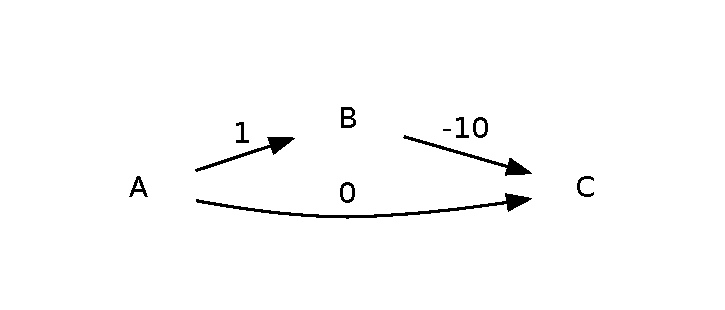
\includegraphics{ex07ex2.pdf}
\caption{Counterexample for Dijkstra with negative weights.
	Attribution: This specific counterexample adapated from stackexchange.}
\label{fig:dijkstraeg}
\end{figure}

It's easy to give a counterexample, once we fix the code.
We prefer to build the heap up-front:
\begin{lstlisting}[numbers=none,xleftmargin=1cm]
dijkstra$(s)$:
	$\pi \gets \text{array}(|V|, \bot)$; $d \gets \text{array}(|V|, \infty)$; $d[s] \gets 0$
	$Q \gets \text{makeheap}(V)$	; priorities $d[v]$
	while $Q \not= \emptyset$
		let $v = \text{deleteMin}(Q)$
		for every $w$ s.t. $v \edge w$	; adj. list
			if $w \in Q$ then
				relax$(v, w)$	% adjusts priority in $Q$
\end{lstlisting}
We omit the evident code for relax.
Now consider what happens when we run this code on the graph in \figref{fig:dijkstraeg} with source $A$.
We dequeue the nodes in order $A$, $C$, $B$, and $D$.
Relaxing from $A$ produces the ``shortest path forest'' (\ie $\pi$ and $d$)
\[
	\Tree [.$0A$ $2D$ $0C$ $1B$ ]
\]
The forest remains unchanged until we relax from $D$ and get
\[
	\Tree [.$0A$ [.$2D$ $-3B$ ] $0C$ ]
\]
This (terminal) forest says that the shortest path from $A$ to $C$ has zero costs and comprises the edge $A \edge C$.
That's wrong.
The shortest path is $A \edge D \edge B \edge C$ with cost $2 - 5 + 1 = -2$.

\end{document}
